%
% $Id: ch02_music
%
%   *******************************************************************
%   * SEE THE MAIN FILE "AllegThesis.tex" FOR MORE INFORMATION.       *
%   *******************************************************************
\chapter{Related Work}\label{ch:music}

This chapter gives a description of what music information retrieval (MIR) is, as well as how
the data has been used by Spotify services, as well as third parties using the Spotify API.
Other applications using the Spotify API are also outlined, and compared to Scottipy.

\section{Music Information Retrieval}
One of the first overviews on MIR \cite{Downie:03} uses seven pieces of information
to analyze each song. These areas are pitch, tempo, harmony, timbre, as well as
editorial information, lyrics, and bibliographic information. The pitch of a song
includes notes, intervals between notes, as well as key. The temporal facet included
the speed of a song, time signature, and pitch and harmonic duration. Harmony refers
to two or more pitches at the same time creating a polyphony of notes. This area
also includes chords and chord progressions. The timbral area includes tone color,
such as the difference in sound quality between a flute and a violin. Orchestration,
or instrument selection, is the most important part of timbre. The editorial section
is mostly performance instructions on music, such as notes for dynamics and
articulations. The textual facet is the lyrics of a piece. The lyrics viewed alone
are usually a good measure of the mood of a song, though they may not be enough to
find a desired melody. The paper mentions an example of this phenomenon between
"God Save the Queen" and "My Country 'tis of Thee", as two songs with the same
melody but different lyrics. The bibliographical facet has little to do with the
actual form of the song, but more meta information about who made the song. This
can include:
\begin{itemize}
  \item song title
  \item composer
  \item arranger
  \item editor
  \item performer
\end{itemize}
and other descriptions about a song, rather than traits garnered from the song. Although these
seven facets include all of the information needed about a song, for comparison purposes a more
nuanced look at individual areas within these groupings would be needed. The paper also includes
looks into systems that use MIR, which can be grouped into either analytic/production, or locating
systems. Analytic and production services focus mostly on the complete digital representation of
music, with a deemphasis on bibliographical information. Projects like this are used to create
comprehensive theoretic analyses of songs. Locating systems are used to quickly retrieve existing
works, such as finding songs based on user criteria and where they can be played.

\section{MIR in Spotify}
The Spotify API offers many different features for songs, which include "danceability",
energy, key, loudness, mode, "speechiness", "acousticness", "instrumentalness", duration,
time signature, "liveness", valence, and tempo \cite{Dev:18}. In addition to the data points mentioned
earlier, Spotify uses many others from The Echo Nest to paint a portrait of a musical
composition. Danceability, valence, energy, and tempo
are all different ways of measuring the mood of a track, typically songs with a happier
mood will have higher values. Loudness, speechiness, and instrumentalness are all properties
of songs, showing how much of a given element is present.  Liveness and acousticness show the
context of a song, so if it is a live recording or an acoustic version.

\section{Related Works}

The Spotify Developer Showcase \cite{Spotify:19} is a collection of submitted
projects that take advantage of various facets of the Spotify API. Since the
API collects information about user listening habits, as well as song data, many
projects focus on using existing user data. One such project is Klarafy
\cite{DeBock:17}, which takes information from a user's playlists, to find
classical music that they are more likely to enjoy. Klarafy's documentation states,

\begin{quote}
Klarafy starts from the relatively plausible premise that someone who loves loud,
fierce metal, is more likely to enjoy a loud, fierce piece by Wagner than soft,
delicate piano music. Klarafy seeks out the affinities, similarities or
connections between your favourite music and classical music.
To arrive at this 'translation', Klarafy scans your playlist for three criteria:
- your favourite music genre (most common genre);
- the musical mood that prevails in your playlist;
- points of departure determined in advance, such as specific instruments,
voice types, etc.
\end{quote}

Klarafy aggregates data from user playlists, and links that data to a
predetermined set of composers and their works. There is no way to get a new
artist if your taste doesn't fit the composer, however, and getting a new
emotion would practically  involve resetting your Spotify profile.

musicScape \cite{Aleksik:18} is another example relying on user data, which
takes recently played tracks for a user, to generate a minimalist landscape from
audio features of the songs. The color and landscape will change, based on track
features from recently played music.

\begin{center}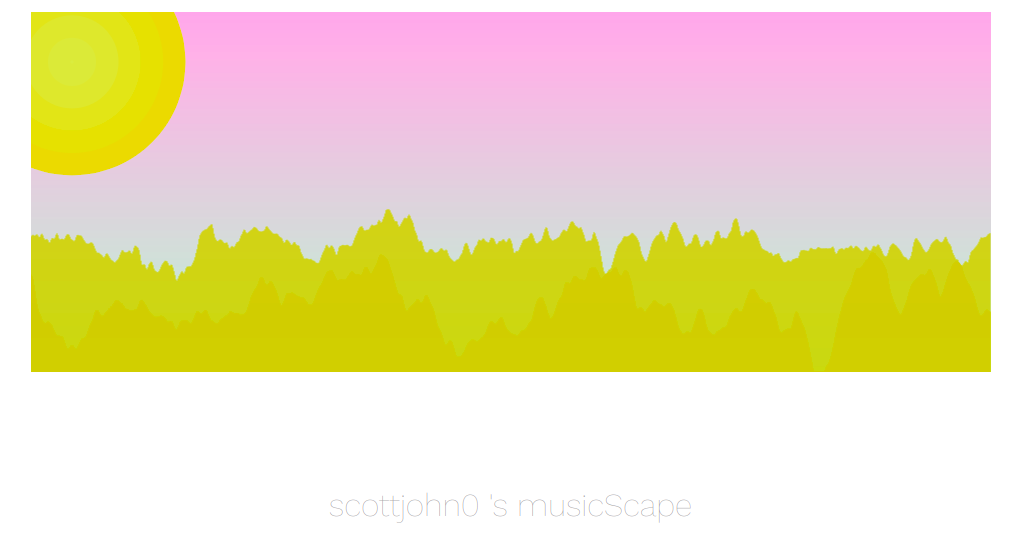
\includegraphics[height=7cm]{images/musicScape.png}
\end{center}

Playlist Souffle \cite{Hammer:18} is another playlist editor, but it works by
swapping out songs in a playlist, and replacing them with tracks either from the
same album, or by the same artist. This tool can be useful to find lesser-known
songs, while still having a connection to songs the user enjoys.

\begin{center}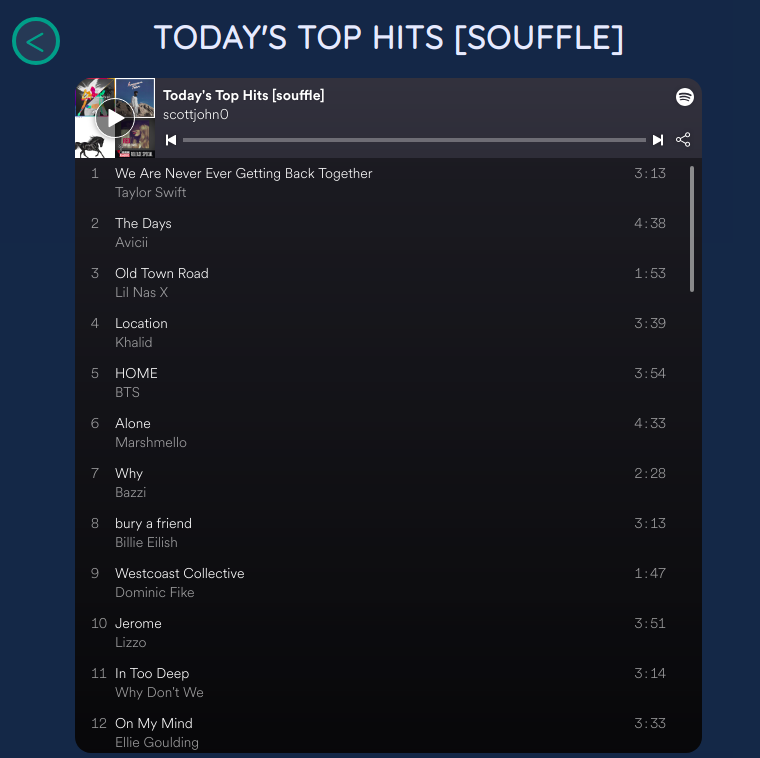
\includegraphics[height=7cm]{images/souffle.png}
\end{center}

The above image is a "souffle" seeded from Spotify's "Today's Top Hits" playlist
\cite{TopHits:19}. The songs have all been changed out, but there is no other
manipulation that can be done. Because of this, the tool is limited as a
"one-and-done", that can only be so effective at finding new music.


Since the spirit of this project is to allow the general public to use the strength
of Spotify's library, and not just established users, projects that do not rely on
user profile data can be more comparable to Scottipy. One of these is MagicPlaylist
\cite{Magic:15}, which is also a web-based playlist creator. The site is much more
limited in its usage of Spotify song data, however; a look through the GitHub source
page \cite{Lovera:15} shows that resulting playlists are based on one aspect of
Spotify artist pages, which is the related artist feature. Because of this,
creating multiple playlists using songs from the same artist as a seed will
give near identical results. In addition to this drawback, there is no way to
edit the resulting list of songs. In tandem, these design decisions create a
rather static experience, which leaves a lot to be desired in terms of creating
an enjoyable collection of music.

Although there are many services using various parts of Spotify's API, no publicly
showcased projects can create playlists based on user chosen criteria, and make
a dynamic result. In the next chapters, I outline how Scottipy seeks to create
a program that meets these challenges.
